\chapter{Gaussian Models}
\label{chap:MVN}

In this chapter, we discuss the \textbf{multivariate Gaussian} or \textbf{multivariate normal(MVN)}, which is the most widely used joint probability density function for continuous variables. It will form the basis for many of the models we will encounter in later chapters.


\section{Basics}
Recall from Section ~\ref{sec:MVN} that the pdf for an MVN in $D$ dimensions is defined by the following:
\begin{equation}
\mathcal{N}(\vec{x}|\vec{\mu},\Sigma) \triangleq \dfrac{1}{(2\pi)^{D/2}|\Sigma|^{1/2}}\exp\left[-\dfrac{1}{2}(\vec{x}-\vec{\mu})^T\Sigma^{-1}(\vec{x}-\vec{\mu})\right]
\end{equation}

The expression inside the exponent is the Mahalanobis distance between a data vector $\vec{x}$ and the mean vector $\vec{\mu}$, We can gain a better understanding of this quantity by performing an \textbf{eigendecomposition} of $\vec{\Sigma}$. That is, we write $\vec{\Sigma}=\vec{U}\vec{\Lambda}\vec{U}^T$, where $\vec{U}$ is an orthonormal matrix of eigenvectors satsifying $\vec{U}^T\vec{U}=\vec{I}$, and $\vec{\Lambda}$ is a diagonal matrix of eigenvalues. Using the eigendecomposition, we have that
\begin{equation}
\vec{\Sigma}^{-1}=\vec{U}^{-T}\vec{\Lambda}^{-1}\vec{U}^{-1}=\vec{U}\vec{\Lambda}^{-1}\vec{U}^T=\sum\limits_{i=1}^D \dfrac{1}{\lambda_i}\vec{u}_i\vec{u}_i^T
\end{equation}
where $\vec{u}_i$ is the $i$’th column of $\vec{U}$, containing the $i$’th eigenvector. Hence we can rewrite the Mahalanobis distance as follows:
\begin{align}
(\vec{x}-\vec{\mu})^T\Sigma^{-1}(\vec{x}-\vec{\mu})& =(\vec{x}-\vec{\mu})^T\left(\sum\limits_{i=1}^D \dfrac{1}{\lambda_i}\vec{u}_i\vec{u}_i^T\right)(\vec{x}-\vec{\mu}) \\
    & =\sum\limits_{i=1}^D \dfrac{1}{\lambda_i}(\vec{x}-\vec{\mu})^T\vec{u}_i\vec{u}_i^T(\vec{x}-\vec{\mu})=\sum\limits_{i=1}^D \dfrac{y_i^2}{\lambda_i}
\end{align}
where $y_i \triangleq \vec{u}_i^T(\vec{x}-\vec{\mu})$. Recall that the equation for an ellipse in 2d is
\begin{equation}
\dfrac{y_1^2}{\lambda_1}+\dfrac{y_2^2}{\lambda_2}=1
\end{equation}

Hence we see that the contours of equal probability density of a Gaussian lie along ellipses. This is illustrated in Figure ~\ref{fig:2d-MVN}. The eigenvectors determine the orientation of the ellipse, and the eigenvalues determine how elogonated it is.

\begin{figure}[hbtp]
\centering
    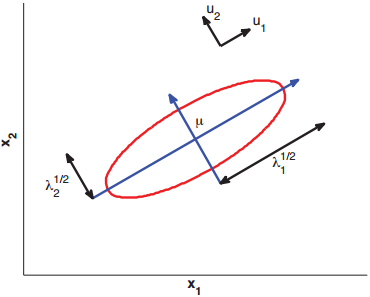
\includegraphics[scale=.70]{2d-MVN.png}
\caption{Visualization of a 2 dimensional Gaussian density. The major and minor axes of the ellipse are defined by the first two eigenvectors of the covariance matrix, namely $\vec{u}_1$ and $\vec{u}_2$. Based on Figure 2.7 of (Bishop 2006a)}
\label{fig:2d-MVN} 
\end{figure}

In general, we see that the Mahalanobis distance corresponds to Euclidean distance in a transformed coordinate system, where we shift by $\vec{\mu}$ and rotate by $\vec{U}$.


\subsection{MLE for a MVN}
\begin{theorem}(\textbf{MLE for a MVN})
If we have $N$ iid samples $\vec{x}_i \sim \mathcal{N}(\vec{\mu},\vec{\Sigma})$, then the MLE for the parameters is given by
\begin{align}
& \bar{\vec{\mu}}=\dfrac{1}{N}\sum\limits_{i=1}^N \vec{x}_i \triangleq \bar{\vec{x}} \\
& \bar{\vec{\Sigma}}=\dfrac{1}{N}\sum\limits_{i=1}^N (\vec{x}_i-\bar{\vec{x}})(\vec{x}_i-\bar{\vec{x}})^T=\dfrac{1}{N}\left(\sum\limits_{i=1}^N \vec{x}_i\vec{x}_i^T\right)-\bar{\vec{x}}\bar{\vec{x}}^T
\end{align}
\end{theorem}


\subsection{Maximum entropy derivation of the Gaussian *}
In this section, we show that the multivariate Gaussian is the distribution with maximum entropy subject to having a specified mean and covariance (see also Section TODO). This is one reason the Gaussian is so widely used: the first two moments are usually all that we can reliably estimate from data, so we want a distribution that captures these properties, but otherwise makes as few addtional assumptions as possible.

To simplify notation, we will assume the mean is zero. The pdf has the form
\begin{equation}
f(\vec{x})=\dfrac{1}{Z}\exp\left(-\dfrac{1}{2}\vec{x}^T\vec{\Sigma}^{-1}\vec{x}\right)
\end{equation}


\section{Gaussian discriminant analysis}
One important application of MVNs is to define the the class conditional densities in a generative classifier, i.e.,
\begin{equation}
p(\vec{x}|y=c,\vec{\theta})=\mathcal{N}(\vec{x}|\vec{\mu}_c,\vec{\Sigma}_c)
\end{equation}

The resulting technique is called (Gaussian) \textbf{discriminant analysis} or \textbf{GDA} (even though it is a generative, not discriminative, classifier — see Section TODO for more on this distinction). If $\vec{\Sigma}_c$ is diagonal, this is equivalent to naive Bayes.

We can classify a feature vector using the following decision rule, derived from Equation ~\eqref{eqn:Generative-classifier}:
\begin{equation}
y=\arg\max_{c} \left[\log p(y=c|\vec{\pi})+\log p(\vec{x}|\vec{\theta})\right]
\end{equation}

When we compute the probability of $\vec{x}$ under each class conditional density, we are measuring the distance from $\vec{x}$ to the center of each class, $\vec{\mu}_c$, using Mahalanobis distance. This can be thought of as a \textbf{nearest centroids classifier}.

\begin{figure}[hbtp]
\centering
    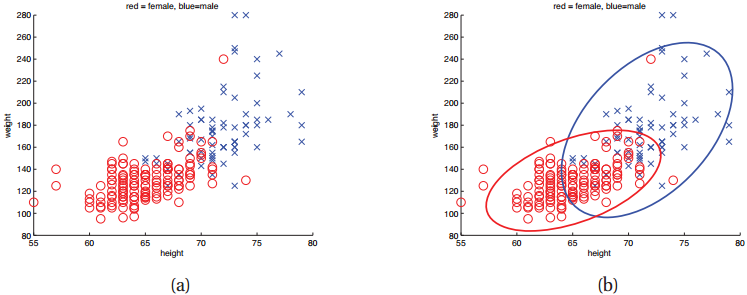
\includegraphics[scale=.70]{2d-Gaussians-Visualization.png}
\caption{(a) Height/weight data. (b) Visualization of 2d Gaussians fit to each class. 95\% of the probability mass is inside the ellipse.}
\label{fig:2d-Gaussians-Visualization} 
\end{figure}

As an example, Figure ~\ref{fig:2d-Gaussians-Visualization} shows two Gaussian class-conditional densities in 2d, representing the height and weight of men and women. We can see that the features are correlated, as is to be expected (tall people tend to weigh more). The ellipses for each class contain 95\% of the probability mass. If we have a uniform prior over classes, we can classify a new test vector as follows:
\begin{equation}
y=\arg\max_{c} (\vec{x}-\vec{\mu}_c)^T\vec{\Sigma}_c^{-1}(\vec{x}-\vec{\mu}_c)
\end{equation}


\subsection{Quadratic discriminant analysis (QDA)}
By plugging in the definition of the Gaussian density to Equation ~\eqref{eqn:Generative-classifier}, we can get
\begin{equation}\label{eqn:QDA}
p(y|\vec{x},\vec{\theta})=\dfrac{\pi_c|2\pi\vec{\Sigma}_c|^{-\frac{1}{2}}\exp\left[-\frac{1}{2}(\vec{x}-\vec{\mu})^T\vec{\Sigma}^{-1}(\vec{x}-\vec{\mu})\right]}{\sum_{c'}\pi_{c'}|2\pi\vec{\Sigma}_{c'}|^{-\frac{1}{2}}\exp\left[-\frac{1}{2}(\vec{x}-\vec{\mu})^T\vec{\Sigma}^{-1}(\vec{x}-\vec{\mu})\right]}
\end{equation}

Thresholding this results in a quadratic function ofx. The result is known as quadratic discriminant analysis(QDA). Figure ~\ref{fig:QDA} gives some examples of what the decision boundaries look like in 2D.

\begin{figure}[hbtp]
\centering
    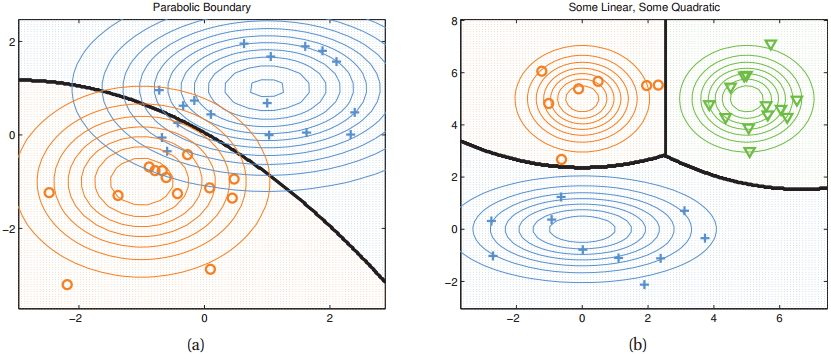
\includegraphics[scale=.60]{QDA.png}
\caption{Quadratic decision boundaries in 2D for the 2 and 3 class case.}
\label{fig:QDA} 
\end{figure}


\subsection{Linear discriminant analysis (LDA)}
\label{sec:Linear-discriminant-analysis}
We now consider a special case in which the covariance matrices are \textbf{tied} or \textbf{shared} across classes,$\vec{\Sigma}_c=\vec{\Sigma}$. In this case, we can simplify Equation ~\eqref{eqn:QDA} as follows:
\begin{align}
p(y|\vec{x},\vec{\theta})& \propto \pi_c\exp\left(\vec{\mu}_c\vec{\Sigma}^{-1}\vec{x}-\dfrac{1}{2}\vec{x}^T\vec{\Sigma}^{-1}\vec{x}-\dfrac{1}{2}\vec{\mu}_c^T\vec{\Sigma}^{-1}\vec{\mu}_c\right) \\
 & =\exp\left(\vec{\mu}_c\vec{\Sigma}^{-1}\vec{x}-\dfrac{1}{2}\vec{\mu}_c^T\vec{\Sigma}^{-1}\vec{\mu}_c+\log \pi_c\right)\exp\left(-\dfrac{1}{2}\vec{x}^T\vec{\Sigma}^{-1}\vec{x}\right) \\
 & \propto \exp\left(\vec{\mu}_c\vec{\Sigma}^{-1}\vec{x}-\dfrac{1}{2}\vec{\mu}_c^T\vec{\Sigma}^{-1}\vec{\mu}_c+\log \pi_c\right)
\end{align}

Since the quadratic term $\vec{x}^T\vec{\Sigma}^{-1}\vec{x}$ is independent of $c$, it will cancel out in the numerator and denominator. If we define
\begin{align}
\gamma_c& \triangleq -\dfrac{1}{2}\vec{\mu}_c^T\vec{\Sigma}^{-1}\vec{\mu}_c+\log \pi_c \\
\vec{\beta}_c& \triangleq \vec{\Sigma}^{-1}\vec{\mu}_c
\end{align}
then we can write
\begin{equation}\label{eqn:LDA}
p(y|\vec{x},\vec{\theta})=\dfrac{e^{\vec{\beta}_c^T\vec{x}+\gamma_c}}{\sum_{c'}e^{\vec{\beta}_{c'}^T\vec{x}+\gamma_{c'}}} \triangleq \sigma(\vec{\eta}, c) \quad \text{where } \vec{\eta} \triangleq (e^{\vec{\beta}_1^T\vec{x}}+\gamma_1,\cdots, e^{\vec{\beta}_C^T\vec{x}}+\gamma_C)
\end{equation}
where $\sigma()$ is the \textbf{softmax activation function}\footnote{\url{http://en.wikipedia.org/wiki/Softmax_activation_function}}, defined as follows:
\begin{equation}
\sigma(\vec{q},i) \triangleq \dfrac{\exp(q_i)}{\sum_{j=1}^n \exp(q_j)}
\end{equation}

When parameterized by some constant, $\alpha > 0$, the following formulation becomes a smooth, differentiable approximation of the maximum function:
\begin{equation}
\mathcal{S}_{\alpha}(\vec{x}) = \dfrac{\sum_{j=1}^D x_je^{\alpha x_j}}{\sum_{j=1}^D e^{\alpha x_j}}
\end{equation}

$\mathcal{S}_{\alpha}$ has the following properties:
\begin{enumerate}
\item $\mathcal{S}_{\alpha} \rightarrow \max$ as $\alpha \rightarrow \infty$
\item $\mathcal{S}_0$ is the average of its inputs
\item $\mathcal{S}_{\alpha} \rightarrow \min$ as $\alpha \rightarrow -\infty$
\end{enumerate}

Note that the softmax activation function comes from the area of statistical physics, where it is common to use the \textbf{Boltzmann distribution}, which has the same form as the softmax activation function.

An interesting property of Equation ~\eqref{eqn:LDA} is that, if we take logs, we end up with a linear function of $\vec{x}$. (The reason it is linear is because the $\vec{x}^T\vec{\Sigma}^{-1}\vec{x}$ cancels from the numerator and denominator.) Thus the decision boundary between any two classes, says $c$ and $c'$, will be a straight line. Hence this technique is called \textbf{linear discriminant analysis} or \textbf{LDA}.

An alternative to fitting an LDA model and then deriving the class posterior is to directly fit $p(y|\vec{x},\vec{W})=\text{Cat}(y|\vec{W}\vec{x})$ for some $C \times D$ weight matrix $\vec{W}$. This is called \textbf{multi-class logistic regression}, or \textbf{multinomial logistic regression}. We will discuss this model in detail in Section TODO. The difference between the two approaches is explained in Section TODO.


\subsection{Two-class LDA}
To gain further insight into the meaning of these equations, let us consider the binary case. In this case, the posterior is given by
\begin{align}
p(y=1|\vec{x},\vec{\theta})& =\dfrac{e^{\vec{\beta}_1^T\vec{x}+\gamma_1}}{e^{\vec{\beta}_0^T\vec{x}+\gamma_0}+e^{\vec{\beta}_1^T\vec{x}+\gamma_1}}) \\
  & =\dfrac{1}{1+e^(\vec{\beta}_0-\vec{\beta}_1)^T\vec{x}+(\gamma_0-\gamma_1)}=\text{sigm}((\vec{\beta}_1-\vec{\beta}_0)^T\vec{x}+(\gamma_0-\gamma_1))
\end{align}
where sigm$(x)$ refers to the sigmoid function\footnote{\url{http://en.wikipedia.org/wiki/Sigmoid_function}}.

Now
\begin{align}
\gamma_1-\gamma_0& = -\dfrac{1}{2}\vec{\mu}_1^T\vec{\Sigma}^{-1}\vec{\mu}_1+\dfrac{1}{2}\vec{\mu}_0^T\vec{\Sigma}^{-1}\vec{\mu}_0 + \log(\pi_1/\pi_0) \\
 & =-\dfrac{1}{2}(\vec{\mu}_1-\vec{\mu}_0)^T\vec{\Sigma}^{-1}(\vec{\mu}_1+\vec{\mu}_0)+ \log(\pi_1/\pi_0)
\end{align}

So if we define
\begin{align}
\vec{w}& =\vec{\beta}_1-\vec{\beta}_0=\vec{\Sigma}^{-1}(\vec{\mu}_1-\vec{\mu}_0) \\
\vec{x}_0& =\dfrac{1}{2}(\vec{\mu}_1+\vec{\mu}_0)-(\vec{\mu}_1-\vec{\mu}_0)\dfrac{\log(\pi_1/\pi_0)}{(\vec{\mu}_1-\vec{\mu}_0)^T\vec{\Sigma}^{-1}(\vec{\mu}_1-\vec{\mu}_0)}
\end{align}
then we have $\vec{w}^T\vec{x}_0=-(\gamma_1-\gamma_0)$, and hence
\begin{equation}
p(y=1|\vec{x},\vec{\theta})=\text{sigm}(\vec{w}^T(\vec{x}-\vec{x}_0))
\end{equation}

(This is closely related to logistic regression, which we will discuss in Section TODO.) So the final decision rule is as follows: shift $\vec{x}$ by $\vec{x}_0$, project onto the line \vec{w}, and see if the result is positive or negative.

\begin{figure}[hbtp]
\centering
    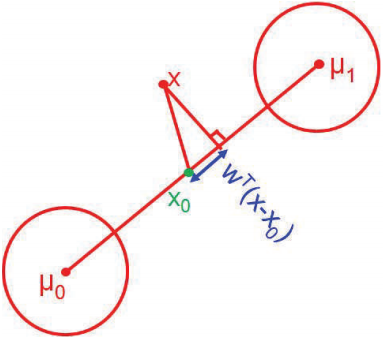
\includegraphics[scale=.60]{2d-LDA.png}
\caption{Geometry of LDA in the 2 class case where $\vec{\Sigma}_1=\vec{\Sigma}_2=\vec{I}$.}
\label{fig:2d-LDA} 
\end{figure}

If $\vec{\Sigma}=\sigma^2\vec{I}$, then $\vec{w}$ is in the direction of $\vec{\mu}_1-\vec{\mu}_0$. So we classify the point based on whether its projection is closer to $\vec{\mu}_0$ or $\vec{\mu}_1$ . This is illustrated in Figure ~\ref{fig:2d-LDA}. Furthemore, if $\vec{\pi}_1=\vec{\pi}_0$, then $\vec{x}_0=\frac{1}{2}(\vec{\mu}_1+\vec{\mu}_0)$, which is half way between the means. If we make $\vec{\pi}_1>\vec{\pi}_0$, then $\vec{x}_0$ gets closer to $\vec{\mu}_0$, so more of the line belongs to class 1 a \emph{priori}. Conversely if $\vec{\pi}_1<\vec{\pi}_0$, the boundary shifts right. Thus we see that the class prior, πc, just changes the decision threshold, and not the overall geometry, as we claimed above. (A similar argument applies in the multi-class case.)

The magnitude of $\vec{w}$ determines the steepness of the logistic function, and depends on how well-separated the means are, relative to the variance. In psychology and signal detection theory, it is common to define the \textbf{discriminability} of a signal from the background noise using a quantity called \textbf{d-prime}:
\begin{equation}
d' \triangleq \dfrac{\mu_1-\mu_0}{\sigma}
\end{equation}
where $\mu_1$ is the mean of the signal and $\mu_0$ is the mean of the noise, and $\sigma$ is the standard deviation of the noise. If $d'$ is large, the signal will be easier to discriminate from the noise.


\subsection{MLE for discriminant analysis}
\label{sec:MLE-for-discriminant-analysis}
The log-likelihood function is as follows:
\begin{equation}
p(\mathcal{D}|\vec{\theta})=\sum\limits_{c=1}^C{\sum\limits_{i:y_i=c}{\log\pi_c}}+\sum\limits_{c=1}^C{\sum\limits_{i:y_i=c}{\log\mathcal{N}(\vec{x}_i|\vec{\mu}_c,\vec{\Sigma}_c)}}
\end{equation}

The MLE for each parameter is as follows:
\begin{align}
\bar{\vec{\mu}}_c& = \dfrac{N_c}{N} \\
\bar{\vec{\mu}}_c& = \dfrac{1}{N_c}\sum\limits_{i:y_i=c}\vec{x}_i \\
\bar{\vec{\Sigma}}_c& = \dfrac{1}{N_c}\sum\limits_{i:y_i=c}(\vec{x}_i-\bar{\vec{\mu}}_c)(\vec{x}_i-\bar{\vec{\mu}}_c)^T
\end{align}


\subsection{Strategies for preventing overfitting}
The speed and simplicity of the MLE method is one of its greatest appeals. However, the MLE can badly overfit in high dimensions. In particular, the MLE for a full covariance matrix is singular if $N_c <D$. And even when $N_c >D$, the MLE can be ill-conditioned, meaning it is close to singular. There are several possible solutions to this problem:
\begin{itemize}
\item{Use a diagonal covariance matrix for each class, which assumes the features are conditionally independent; this is equivalent to using a naive Bayes classifier (Section ~\ref{sec:NBC})}.
\item{Use a full covariance matrix, but force it to be the same for all classes,$\vec{\Sigma}_c=\vec{\Sigma}$. This is an example of \textbf{parameter tying} or \textbf{parameter sharing}, and is equivalent to LDA (Section ~\ref{sec:Linear-discriminant-analysis}).}
\item{Use a diagonal covariance matrix and forced it to be shared. This is called diagonal covariance LDA, and is discussed in Section TODO.}
\item{Use a full covariance matrix, but impose a prior and then integrate it out. If we use a conjugate prior, this can be done in closed form, using the results from Section TODO; this is analogous to the “Bayesian naive Bayes” method in Section ~\ref{sec:Bayesian-naive-Bayes}. See (Minka 2000f) for details.}
\item{Fit a full or diagonal covariance matrix by MAP estimation. We discuss two different kindsof prior below.}
\item{Project the data into a low dimensional subspace and fit the Gaussians there. See Section TODO for a way to find the best (most discriminative) linear projection.}
\end{itemize}

We discuss some of these options below.


\subsection{Regularized LDA *}


\subsection{Diagonal LDA}


\subsection{Nearest shrunken centroids classifier *}
One drawback of diagonal LDA is that it depends on all of the features. In high dimensional problems, we might prefer a method that only depends on a subset of the features, for reasons of accuracy and interpretability. One approach is to use a screening method, perhaps based on mutual information, as in Section 3.5.4. We now discuss another approach to this problem known as the \textbf{nearest shrunken centroids} classifier (Hastie et al. 2009, p652).


\section{Inference in jointly Gaussian distributions}
\label{sec:Inference-in-jointly-Gaussian-distributions}
Given a joint distribution, $p(\vec{x}_1,\vec{x}_2)$, it is useful to be able to compute marginals $p(\vec{x}_1)$ and conditionals $p(\vec{x}_1|\vec{x}_2)$. We discuss how to do this below, and then give some applications. These operations take $O(D^3)$ time in the worst case. See Section TODO for faster methods.


\subsection{Statement of the result}

\begin{theorem}(\textbf{Marginals and conditionals of an MVN}). Suppose $X=(\vec{x}_1,\vec{x}_2)$is jointly Gaussian with parameters
\begin{equation}
\vec{\mu}=\left(\begin{array}{c}\vec{\mu}_1 \\
                                \vec{\mu}_2\end{array}\right),
\vec{\Sigma}=\left(\begin{array}{cc}
                   \vec{\Sigma}_{11} & \vec{\Sigma}_{12} \\
 				   \vec{\Sigma}_{21} & \vec{\Sigma}_{22} \end{array}\right),
\vec{\Lambda}=\vec{\Sigma}^{-1}=\left(\begin{array}{cc}
                   \vec{\Lambda}_{11} & \vec{\Lambda}_{12} \\
 				   \vec{\Lambda}_{21} & \vec{\Lambda}_{22} \end{array}\right),
\end{equation}

Then the marginals are given by
\begin{equation}
\begin{split}
p(\vec{x}_1)= \mathcal{N}(\vec{x}_1|\vec{\mu}_1,\vec{\Sigma}_{11})\\
p(\vec{x}_2)= \mathcal{N}(\vec{x}_2|\vec{\mu}_2,\vec{\Sigma}_{22})
\end{split}
\end{equation}
and the posterior conditional is given by
\begin{equation}\label{eqn:Marginals-and-conditionals-of-an-MVN}
  \boxed{\begin{split}
    p(\vec{x}_1|\vec{x}_2)& =\mathcal{N}(\vec{x}_1|\vec{\mu}_{1|2},\vec{\Sigma}_{1|2}) \\
    \vec{\mu}_{1|2}& = \vec{\mu}_1+\vec{\Sigma}_{12}\vec{\Sigma}_{22}^{-1}(\vec{x}_2-\vec{\mu}_2) \\
	               & = \vec{\mu}_1-\vec{\Lambda}_{11}^{-1}\vec{\Lambda}_{12}(\vec{x}_2-\vec{\mu}_2) \\
				   & = \vec{\Sigma}_{1|2}(\vec{\Lambda}_{11}\vec{\mu}_1-\vec{\Lambda}_{12}(\vec{x}_2-\vec{\mu}_2)) \\
	\vec{\Sigma}_{1|2}& = \vec{\Sigma}_{11}-\vec{\Sigma}_{12}\vec{\Sigma}_{22}^{-1}\vec{\Sigma}_{21}=\vec{\Lambda}_{11}^{-1}
  \end{split}}
\end{equation}
\end{theorem}

Equation ~\eqref{eqn:Marginals-and-conditionals-of-an-MVN} is of such crucial importance in this book that we have put a box around it, so you can easily find it. For the proof, see Section TODO.

We see that both the marginal and conditional distributions are themselves Gaussian. For the marginals, we just extract the rows and columns corresponding to $\vec{x}_1$ or $\vec{x}_2$. For the conditional, we have to do a bit more work. However, it is not that complicated: the conditional mean is just a linear function of $\vec{x}_2$, and the conditional covariance is just a constant matrix that is independent of $\vec{x}_2$. We give three different (but equivalent) expressions for the posterior mean, and two different (but equivalent) expressions for the posterior covariance; each one is useful in different circumstances.


\subsection{Examples}
Below we give some examples of these equations in action, which will make them seem more intuitive.


\subsubsection{Marginals and conditionals of a 2d Gaussian}



